\documentclass{article}
\usepackage[utf8]{inputenc}
\usepackage[english]{babel}
\usepackage[]{amsthm}
\usepackage[]{amssymb}
\usepackage[]{amsmath}
\usepackage[]{graphicx}
\usepackage[]{hyperref}
\usepackage[]{xcolor}
\usepackage[]{cancel}
\usepackage[]{fancyhdr}
\hypersetup{
    colorlinks,
    linkcolor={red!50!black},
    citecolor={blue!50!black},
    urlcolor={blue!80!black}
}

\pagestyle{fancy}
\fancyhf{}
\title{\vspace{-4cm}MTH20012 - Series and Transformations Test 2}
\author{Joshua Rogers}
\lhead{MTH20012 Test 2}
\rhead{Joshua Rogers 101096819}
\date\today

\begin{document}
\maketitle 

\section*{Part B Question 5}

\[ f(t) = \begin{cases} 
      4 & 0\leq t < 6 \\
      -\frac{5}{6}t+9 & 6\leq t < 12
   \end{cases}
\]

\subsection*{A}

We let $u=t$ and $dv=cos(at)$, thus $du = 1$ and $v = \frac{sin(at)}{a}$
\begin{align*}
\int t cos(at) dt =&\\
&\frac{tsin(at)}{a} - \int \frac{sin(at)}{a} dt\\
= &\frac{tsin(at)}{a} + \frac{cos(at)}{a^2}
\end{align*}

\subsection*{B}

We let $u=t$ and $dv=sin(at)$, thus $du = 1$ and $v = -\frac{cos(at)}{a}$
\begin{align*}
\int t sin(at) dt =&\\
&-\frac{tcos(at)}{a} - \int -\frac{cos(at)}{a} dt\\
= &-\frac{tcos(at)}{a} + \frac{sin(at)}{a^2}
\end{align*}

\subsection*{C}
See image below.
\begin{figure}
\centering
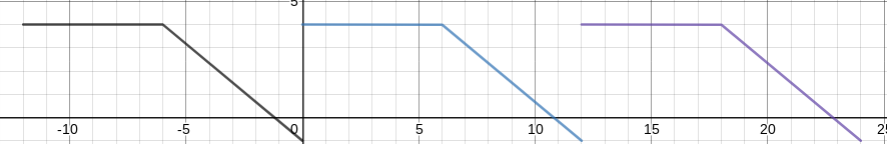
\includegraphics[width=1.0\textwidth]{./static/graph3.png}
\caption{Part C}
\end{figure}

\pagebreak

\subsection*{D}

We define the function

\[ f(t) = \begin{cases}
      4 & 0\leq t < 6 \\
      -\frac{5}{6}t+9 & 6\leq t < 12 \\
      f(t + 12) & \forall t
   \end{cases}
\]


$$a_n = \frac{2}{T} \int_{0}^{T} f(t) cos(n\omega t) dt$$
$$b_n = \frac{2}{T} \int_{0}^{T} f(t) sin(n\omega t) dt$$
$$\omega = 2\pi/T$$
$$T = 12$$

Solving for $a_0$ we obtain   
$$a_0 = \frac{1}{6} \left[ \int_{0}^{6} 4dt + \int_6^{12} \frac{-5}{6} t + 9dt \right ] = \frac{11}{2}$$

Solving for $a_n$:
$$\frac{12}{2}a_n =  \int_{0}^{6} 4\cdot cos\left(\frac{n\cdot \pi\cdot t}{6}\right) dt + \int_{6}^{12} \left(-\frac{5t}{6} + 9\right) \cdot cos\left(\frac{n\cdot \pi\cdot t}{6}\right)dt$$
$$6a_n =  4\int_{0}^{6} cos\left(\frac{n\cdot \pi\cdot t}{6}\right) dt + 9 \int_{6}^{12} cos\left(\frac{n\cdot \pi\cdot t}{6}\right)dt + \frac{-5}{6} \int_{6}^{12} t\cdot cos\left(\frac{n\cdot \pi\cdot t}{6}\right)dt$$

Using the solution to the integral found previously with $a=\frac{n\cdot \pi}{6}$ we obtain
$$6a_n =  4\int_{0}^{6} cos\left(\frac{n\cdot \pi\cdot t}{6}\right) dt + 9 \int_{6}^{12} cos\left(\frac{n\cdot \pi\cdot t}{6}\right)dt + \frac{-5}{6}
\left[ \int_{6}^{12} t\cdot cos\left(\frac{n\cdot \pi\cdot t}{6}\right)dt\right]$$

\begin{align*}
6a_n =  4\int_{0}^{6} cos\left(\frac{n\cdot \pi\cdot t}{6}\right) dt + 9 \int_{6}^{12} cos\left(\frac{n\cdot \pi\cdot t}{6}\right)dt + \\
&\frac{-5}{6} \left[ \frac{36cos\left(\frac{12 \pi n}{6}\right)}{\pi^2n^2} + \frac{6 \cdot 12 \cdot sin\left(\frac{12 \pi n}{6}\right)}{\pi n} \right ] - \\
&\frac{-5}{6} \left[ \frac{36cos\left(\frac{6 \cdot \pi n}{6}\right)}{\pi^2n^2} + \frac{6 \cdot 6 \cdot sin\left(\frac{6 \cdot \pi n}{6}\right)}{\pi n} \right]
\end{align*}

Thus, we have

$$
6a_n = \frac{24 sin(\pi n)}{\pi n} + \frac{54sin(2 \pi n) - sin(\pi n))}{\pi n} - \frac{5}{6} \left[ \frac{36cos\left(2 \pi n\right)}{\pi^2n^2} + \frac{72 \cdot sin\left(2 \pi n\right)}{\pi n} \right ] + \frac{5}{6} \left[ \frac{36cos\left(\pi n\right)}{\pi^2n^2} + \frac{36 \cdot sin\left(\pi n\right)}{\pi n} \right]
$$

The $sin$ terms cancel go to zero and we are left with
$$ a_n = \frac{5(cos(\pi n) - cos(2 \pi n))}{\pi^2n^2}$$
or rather
$$
a_n = \frac{5}{\pi^2n^2} \left[ \left(-1\right)^n - 1 \right]
$$

Noting that the even terms here are 0, we let $n=2n+1$ and thus obtain
$$
a_{2n+1} = \frac{-10}{\left(2n+1\right)^2\pi^2}
$$


Similarly for $b_n$, we obtain
$$\frac{4}{\pi n} + \frac{cos(2\pi n)}{\pi n}$$
or rather
$$
b_n = \frac{5}{\pi n}
$$

Thus we have our full-range Fourier series for $f(t)$.

$$
f(t) \sim \frac{11}{4} + \sum_{n=1}^{\infty}\frac{5}{\pi n}\sin\left(\frac{n\pi t}{6}\right)+\sum_{n=0}^{\infty}\frac{-10}{\left(2n+1\right)^{2}\pi^{2}}\cos\left(\frac{\left(2n+1\right)\pi t}{6}\right)
$$
\subsection*{E}

See image above.
\begin{figure}
\centering
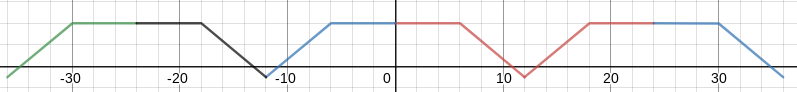
\includegraphics[width=1.0\textwidth]{./static/graph4.png}
\caption{Part E}
\end{figure}


\subsection*{F}


We define the function

\[ f_e(t) = \begin{cases}
      4 & 0\leq t < 6 \\
      -\frac{5}{6}t+9 & 6\leq t < 12 \\
      4 & -6\leq t < 0 \\
      \frac{5}{6}t+9 & -12 \leq t < -6 \\
      f_e(t + 24) & \forall t
   \end{cases}
\]

We have $T=24$ and $b_n=0$ for all $n$ and $\omega = \frac{2\pi}{24} = \frac{\pi}{12}$

We have already shown we know how to do integration by parts so ignore quite a lot of working.

$$
a_0 = \frac{4}{24} \left[ \int_0^6 4 dt + \int_6^{12} \frac{-5t}{6} + 9 dt \right] = \frac{11}{2}
$$

$$
\frac{a_n}{2} = \frac{2}{24} \left[ \int_0^{6} 4 cos\left( \frac{n \pi t}{12} \right) dt + \int_6^{12} cos\left(\frac{n \pi t}{12}\right)\left(\frac{-5t}{6}+9\right)dt\right]
$$
The $\frac{1}{2}$ by the $a_n$ arises from the symmetric nature of the even periodic extension of the function.

Through the same rigorous task as seen in previous part, we obtain

$$
\frac{a_n}{2} = \frac{-sin(\pi n)}{\pi n} - \frac{10cos(\pi n)}{\pi^2 n^2} + \frac{10cos(\frac{\pi n}{2})}{\pi^2 n^2}
$$

Thus,
$$
a_n =\frac{20}{\pi^2n^2} \left[ \left(-1\right)^{n+1} +cos\left(\frac{\pi n}{2}\right) \right]
$$

Noting that $cos\left(\frac{\pi n}{2}\right)$ is zero for odd numbers of $n$, we let $n=2n$ for the second part and obtain

$$
a_n  =\frac{20}{\pi^2n^2} \left(-1\right)^{n+1}
$$
and
$$
a_{2n} = \frac{5}{\pi^2 n^2} \left(-1\right)^{n}
$$

Thus we have

$$
f_e(t) \sim \frac{11}{4}+\sum_{n=1}^{\infty}\frac{20}{n^{2}\pi^{2}}\left(-1\right)^{\left(n+1\right)}\cos\left(\frac{n\pi t}{12}\right) + \sum_{n=1}^{\infty}\frac{5}{n^{2}\pi^{2}}\left(-1\right)^{n}\cos\left(\frac{n\pi t}{6}\right)
$$

\subsection*{G}

See image above.

\begin{figure}
\centering
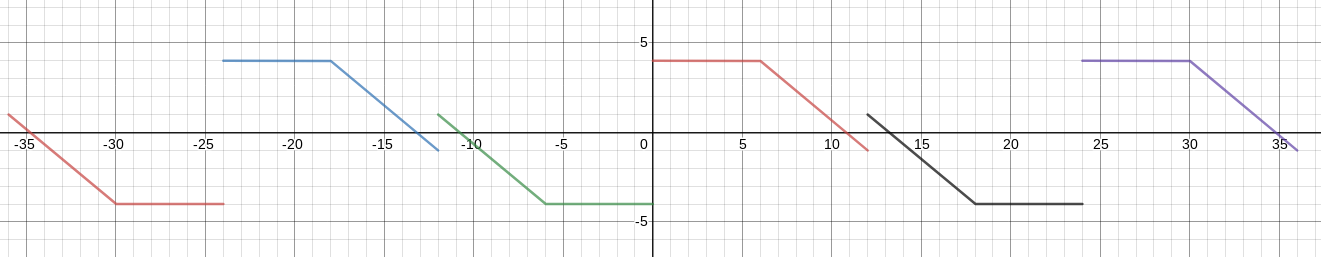
\includegraphics[width=1.0\textwidth]{./static/graph5.png}
\caption{Part G}
\end{figure}

\subsection*{H}

We define the function

\[ f_o(t) = \begin{cases}
      4 & 0\leq t < 6 \\
      -\frac{5}{6}t+9 & 6\leq t < 12 \\
      -4 & -6\leq t < 0 \\
      -\frac{5}{6}t-9 & -12 \leq t < -6 \\
      f_o(t + 24) & \forall t
   \end{cases}
\]  

We have the exact same as part F, however $a_0=0$ and $a_n=0$.

We have $T=24$ and $b_n=0$ for all $n$ and $\omega = \frac{2\pi}{24} = \frac{\pi}{12}$

$f_o(t)$ is by definition odd, and $sin(t)$ is odd, thus the integrand is an even function, thus we simply integrate one side and multiply it by two.

$$
b_n = \frac{1}{6} \left[ \int_0^{6} 4 sin\left( \frac{n \pi t}{12} \right) dt + \int_6^{12} sin\left(\frac{n \pi t}{12}\right)\left(\frac{-5t}{6}+9\right)dt\right]
$$

$$
b_n = \frac{2}{\pi^2n^2} \left( 4\pi n + \pi n \left(-1\right)^n + 10sin\left(\frac{\pi n}{2}\right)\right)
$$

Noting that the second part is zero for even $n$, we split it up and obtain

$$
b_n = \frac{2}{\pi n} \left[\left(-1\right)^n+4\right]
$$

$$
b_{2n+1} = \frac{20\left(-1\right)^n}{\pi^2\left(2n+1\right)^2}
$$
Thus we have

$$
f_o(t) \sim \sum_{n=1}^{\infty} \frac{2\left[\left(-1\right)^n+4\right]}{\pi n} sin\left(\frac{n \pi t}{12}\right) + \sum_{n=0}^{\infty} \frac{20\left(-1\right)^n}{\pi^2\left(2n+1\right)^2} sin\left(\frac{\left(2n+1\right) \pi t}{12}\right)
$$


\subsection*{I}

The even extension converges fastest.  This is because there is the smallest discontinuity (it is continuous.)
Likewise, plotting all three options on desmos, it is clear that the even extension converges faster; $a=4$ is sufficient compared to $a \approx 40$ for the others.
See: \href{https://www.desmos.com/calculator/1twteyxxyg}{even}, \href{https://www.desmos.com/calculator/ao6mjhce0y}{odd}, \href{https://www.desmos.com/calculator/bk2vlfzv0c}{full}.

\end{document}
